\clearpage
\maketitlesupplementary

% ============================================================
% A. Exact prompts and decoding
% ============================================================
\section{Exact Prompts, Decoding, and Parsing}
\label{app:prompts}

\textbf{VSR plain prompt} (identical for 2B and 7B, all conditions;
`\{statement\}' is the VSR caption):
\begin{verbatim}
Look at the image carefully.

Statement: "{statement}"

Is this statement true or false?

Answer with exactly one word:
True or False.
\end{verbatim}

\textbf{2B structured-decomposition prompt} (2B only; single run):
\begin{verbatim}
Look carefully at the image.

Statement:
"{statement}"

Determine whether the statement is true
by doing the following:
1. Identify the subject object.
2. Identify the reference object.
3. Determine the position and
   orientation of the subject relative
   to the reference object.
4. Pay careful attention to left/right,
   front/back, viewpoint, and
   orientation.
5. Decide whether the stated spatial
   relationship matches the image.

Answer with exactly one word:
True or False.
\end{verbatim}

\textbf{SITE multiple-choice prompt} (replicated from the official
lmms-eval task \texttt{sitebench/utils.py}):
\begin{verbatim}
# image examples (one <image> token per visual):
<image>...
Question: {question}
Options:
A: {opt0}
B: {opt1}
...
Give me the answer letter directly.
The best answer is:

# video examples (pre-prompt):
Select the best answer to the following
multiple-choice question based on the
video. Respond with only the letter
of the correct option.
Question: {question}
Options:
A: ...
B: ...
...
Give me the answer letter directly.
The best answer is:
\end{verbatim}

\textbf{Decoding.} All generations are greedy: $\mathrm{do\_sample}{=}$False,
temperature 0, top-$p$ 1.0. $\mathrm{max\_new\_tokens}$: 5 for the 2B wrapper,
128 for 7B VSR runs, 16 for SITE (change validated parse-identical on 125/125
held-out outputs before adoption; recorded in the SITE run metadata).

\textbf{Parsing.} VSR outputs are parsed with an anchored case-insensitive
regex (\texttt{src/evaluation/parser.py}): strips prefixes
(`the answer is', `answer:', `response:', `output:') and trailing
punctuation; accepts exact `true/yes/correct' or `false/no/incorrect' forms;
substring fallback only when exactly one of `true'/'false' appears. Invalid
outputs are counted as wrong, never guessed; invalid rate is 0 on all reported
runs. SITE outputs use the official \texttt{parse\_multi\_choice\_response}
(letter); unparseable responses are counted incorrect and reported.

% ============================================================
% B. Training configurations
% ============================================================
\section{Training and Adapter Configurations}
\label{app:training}

All LoRA conditions share: $r{=}8$, $\alpha{=}16$, dropout 0.05, AdamW
lr $10^{-4}$, weight decay 0.01, linear warmup 10\% of steps, 2 epochs,
bf16, gradient checkpointing, gradient clipping 1.0, vision tower frozen.
Adapter configs are committed at \texttt{checkpoints/*/final/adapter\_config.json}.

\begin{table*}[h]
\centering
\footnotesize
\setlength{\tabcolsep}{4pt}
\begin{tabular}{llccc}
\toprule
Condition & LoRA targets & Trainable & Batch & Manifest \\
\midrule
2B General & LM q/k/v/o & $\sim$2.3M & microbatch 4$\times$4 & general (2{,}000) \\
2B Targeted & LM q/k/v/o & $\sim$2.3M & same & targeted (2{,}000) \\
7B LM-only & LM q/k/v/o & $\sim$0.3M & 1 & general (2{,}000) \\
7B HardNeg & LM q/k/v/o & $\sim$0.3M & 1 & hard-negative (2{,}000) \\
7B Projector & \texttt{visual.merger.mlp.0/2} & 152K & 1 & general (2{,}000) \\
7B Vision+Proj & merger + blocks 24--31 & 1.46M & 1 & general (2{,}000) \\
\bottomrule
\end{tabular}
\caption{LoRA conditions and their target modules.}
\label{tab:adapters}
\end{table*}

\textbf{Manifest construction.} \emph{General}: 2{,}000 statements sampled from
the VSR train split. \emph{Targeted}: orientation-over-sampled subset of the
same split. \emph{Hard-negative}: the orientation block of the general manifest
is replaced by audited-clean originals plus paired hard negatives
(facing$\leftrightarrow$facing away from; parallel$\leftrightarrow$perpendicular)
with flipped labels; every included example was audited for label correctness
(451 train orientation examples audited: 402 clean, 28 excluded, 21 original-only). 2B runs split
5\% of the manifest for validation (seed 42). All manifests derive exclusively
from the VSR \emph{train} split; all evaluations use \emph{test} only.

% ============================================================
% C. Probe methodology and full tables
% ============================================================
\section{Probe Methodology and Full Tables}
\label{app:probes}

\textbf{Features.} Qwen2-VL-7B-Instruct, vision tower frozen. ViT patch
embeddings (1280-d) and post-merger features (3584-d), mean-pooled per image
(ungrounded) or per grounding box (grounded). Grounding boxes from frozen
Qwen2-VL grounding (94.6\% of 647 orientation images yield both boxes; failures
are mostly genuinely absent objects), rescaled to pixels; region features
mean-pooled over patch centers inside each box.

\textbf{Tasks.} T1 facing vs.\ facing away (test $n{=}103$, majority 64.2\%);
T2 parallel vs.\ perpendicular ($n{=}34$, majority 64.7\%); T3 4-way
($n{=}137$, majority 49.6\%). Training on audited-clean VSR train; 5-fold CV;
no test examples in training.

\textbf{Readouts.} Linear logistic regression; MLP (256 hidden, ReLU, Adam,
early stopping on CV); patch-vote (per-patch linear probe, majority vote over
patches); grounded variants with feature sets \texttt{visual}
($[\text{subj},\text{ref},\text{subj}-\text{ref},\text{subj}\cdot\text{ref}]$),
\texttt{geometry} (12-d normalized box features), and \texttt{visual+geometry}.

\textbf{Ungrounded results} (test acc \%; balanced acc in parentheses; Wilson
95\% CI; majority baselines: T1 64.2\%, T2 64.7\%, T3 49.6\%):
\begin{center}
\footnotesize
\begin{tabular}{lccc}
\toprule
T1 facing vs.\ away ($n{=}103$) & Test & Bal.\ acc & 95\% CI \\
\midrule
ViT linear & 65.0 & 60.4 & $[55, 74]$ \\
ViT MLP & 55.3 & 52.0 & $[45, 65]$ \\
Merger linear & 68.9 & 64.5 & $[59, 77]$ \\
Merger MLP & 52.4 & 49.2 & $[42, 62]$ \\
ViT patch-vote & 62.1 & --- & $[53, 71]$ \\
Merger patch-vote & 60.2 & --- & $[51, 69]$ \\
\bottomrule
\end{tabular}
\end{center}
\begin{center}
\footnotesize
\begin{tabular}{lccc}
\toprule
T2 parallel vs.\ perpendicular ($n{=}34$) & Test & Bal.\ acc & 95\% CI \\
\midrule
ViT linear & 61.8 & 61.0 & $[44, 77]$ \\
ViT MLP & 67.6 & 69.3 & $[50, 82]$ \\
Merger linear & 64.7 & 61.4 & $[47, 79]$ \\
Merger MLP & 64.7 & 63.3 & $[47, 79]$ \\
ViT patch-vote & \textbf{73.5} & --- & $[57, 85]$ \\
Merger patch-vote & 67.6 & --- & $[51, 81]$ \\
\bottomrule
\end{tabular}
\end{center}
\begin{center}
\footnotesize
\begin{tabular}{lccc}
\toprule
T3 4-way ($n{=}137$) & Test & Bal.\ acc & 95\% CI \\
\midrule
ViT linear & 52.6 & 40.5 & $[44, 61]$ \\
ViT MLP & 52.6 & 42.9 & $[44, 61]$ \\
Merger linear & 53.3 & 44.0 & $[45, 61]$ \\
Merger MLP & 47.4 & 43.2 & $[39, 56]$ \\
ViT patch-vote & 51.8 & --- & $[44, 60]$ \\
Merger patch-vote & 52.6 & --- & $[44, 61]$ \\
\bottomrule
\end{tabular}
\end{center}

\textbf{Grounded results} (CV acc / test acc; majority T1 63.7\%,
T2 57.0\%; visual $=[\text{subj},\text{ref},\text{subj}-\text{ref},
\text{subj}\cdot\text{ref}]$; geometry $=$ 12-d box features; T3 4-way is at
chance for every readout, test acc 41.7--52.8\% across all 12 cells vs.\
49.9\% majority, committed JSON):
\begin{center}
\footnotesize
\begin{tabular}{lcccl}
\toprule
Readout & T1 visual & T1 geom.\ & T2 visual & T2 geom.\ \\
\midrule
ViT linear & 59.8/61.6 & 61.1/60.6 & 51.2/53.6 & 44.2/50.0 \\
ViT MLP & 59.5/66.7 & 61.8/62.6 & 45.4/46.4 & 45.4/46.4 \\
Merger linear & 57.2/65.7 & 61.1/60.6 & 51.2/53.6 & 44.2/50.0 \\
Merger MLP & 56.3/52.5 & \textbf{61.1/71.7} & 49.0/53.6 & 50.0/42.9 \\
\bottomrule
\end{tabular}
\end{center}
The single above-majority cell (geometry-only merger MLP on T1, 71.7\% test)
has CV 61.1\% below the 63.7\% majority --- not robust --- and derives from the
grounding model's own box statistics, not vision-feature content. In short,
object-box conditioning with the model's own grounding predictions and
mean-pooled region features does not recover robust orientation decodability
under the tested readouts. The T2 patch-vote result (73.5\%) is a suggestive
point estimate with a wide CI overlapping the majority baseline ($n{=}34$).

\textbf{Clear-subset control (canonical, frozen at \texttt{paper-freeze-v1}).}
The 48-example manual audit identified ambiguous or questionable orientation
labels. Re-evaluation on progressively stricter subsets (values \% from
\texttt{results/tables/orientation\_clean\_label\_table.md}, generated by
\texttt{scripts/clean\_label\_orientation.py}):
\begin{table*}[h]
\centering
\footnotesize
\caption{Clean-label orientation robustness (canonical, frozen at
\texttt{paper-freeze-v1}; values \% from
\texttt{results/tables/orientation\_clean\_label\_table.md}).}
\label{tab:cleanlabel}
\begin{tabular}{lcccc}
\toprule
Condition & Full (137) & $-$Questionable (132) & Clear (124) & Strict (107) \\
\midrule
2B zero-shot & 62.8 & 65.2 & 66.9 & 75.7 \\
2B structured & 53.3 & 52.3 & 51.6 & 53.3 \\
2B General LoRA & 62.0 & 63.6 & 64.5 & 72.9 \\
2B Targeted LoRA & 64.2 & 65.9 & 68.5 & 76.6 \\
7B zero-shot & 63.5 & 65.2 & 68.5 & 72.0 \\
7B General LoRA & 65.7 & 67.4 & 70.2 & \textbf{78.5} \\
7B Targeted LoRA & 64.2 & 65.9 & 69.4 & 72.0 \\
7B Hard-Neg LoRA & \textbf{66.4} & \textbf{68.2} & \textbf{70.2} & 76.6 \\
7B Projector LoRA & 64.2 & 65.9 & 69.4 & 73.8 \\
7B Vision+Projector LoRA & 64.2 & 65.2 & 68.5 & 73.8 \\
\bottomrule
\end{tabular}
\end{table*}
Because auditing changes the evaluated sample, strict-subset values are not a
matched comparison against other relation families. The earlier probe-side
clear/strict check (pre-freeze) additionally suggested that removing
audit-flagged examples does not change the probe conclusion: the best
ungrounded probe moved only
68.9\% $\rightarrow$ 71.1\% $\rightarrow$ 71.6\% (full/clear/strict,
$n=103/97/88$) and the generative T1 readouts 64.1/66.0/68.2 (zero-shot) and
68.9/72.2/78.4 (General LoRA); committed in
\texttt{results/probe/clear\_subset\_results.json}.

% ============================================================
% D. Statistical appendix
% ============================================================
\section{Complete Statistical Test Battery}
\label{app:stats}

All pairwise tests are exact McNemar tests (binomial test on discordant pairs,
two-sided). Discordant counts are reported as (condition-loses /
condition-gains) relative to the control named in each row. No test was run and
withheld; the battery below is complete for this paper.

\begin{table*}[h]
\centering
\footnotesize
\setlength{\tabcolsep}{6pt}
\begin{tabular}{llccc}
\toprule
ID & Comparison & Subset & Discord.\ & $p$ \\
\midrule
1 & HardNeg vs.\ Gen. & overall (2195) & 52/60 & 0.508 \\
2 & HardNeg vs.\ Gen. & weak families & 20/26 & 0.461 \\
3 & Projector vs.\ ctrl. & overall & --- & 0.0043 \\
4 & V+Proj vs.\ ctrl. & overall & --- & 0.0122 \\
5 & Projector vs.\ ctrl. & orientation & --- & 0.86 \\
6 & V+Proj vs.\ ctrl. & orientation & --- & 0.85 \\
7--14 & Proj./V+Proj vs.\ ctrl. & per-relation (4$\times$2) & --- & 0.25--1.00 \\
15 & Two-stage A-lin. vs.\ ctrl. & agreement (127 boxed) & 45/16 & 0.0003 \\
16 & Two-stage A-MLP vs.\ ctrl. & agreement (127 boxed) & 47/14 & $<$0.0001 \\
17 & Two-stage B-lin. vs.\ ctrl. & agreement (127 boxed) & 44/20 & 0.0037 \\
18 & Two-stage B-MLP vs.\ ctrl. & agreement (127 boxed) & 47/18 & 0.0004 \\
19 & Zero-shot vs.\ LM-only & consistency 662 & 117/43 & $<$0.0001 \\
20 & HardNeg vs.\ LM-only & consistency 662 & 31/41 & 0.29 \\
21 & Projector vs.\ LM-only & consistency 662 & 63/48 & 0.18 \\
22 & V+Proj vs.\ LM-only & consistency 662 & 65/56 & 0.47 \\
\bottomrule
\end{tabular}
\caption{Complete VSR test battery (22 rows). Per-relation cells (IDs 7--14)
are enumerated in the committed \texttt{vision\_side\_\allowbreak{}comparison.\allowbreak{}json}:
projector facing $p{=}0.77$, facing-away $p{=}1.00$, parallel $p{=}0.25$,
perpendicular $p{=}1.00$; vision+proj facing $p{=}1.00$, facing-away
$p{=}0.58$, parallel $p{=}1.00$, perpendicular $p{=}1.00$. Rows 15--18 are
\emph{agreement-based}: the committed two-stage pipeline scored agreement
with the control's verdicts (not accuracy against ground truth), so these
rows are descriptive and are excluded from the confirmatory set and from the
Holm family. SITE transfer tests (3: all/primary/secondary, \S E) form a
separate small family.}
\label{tab:tests}
\end{table*}

\textbf{Principal vs.\ exploratory comparisons.} The battery above is fully
enumerated; no test was run and withheld. The \emph{principal}
(confirmatory) comparisons are: zero-shot vs.\ LM-only consistency (ID 19)
and the SITE transfer tests (\S E). All other comparisons --- vision-side
conditions and their per-relation cells, hard-negative training vs.\ control,
the remaining consistency comparisons, and the two-stage agreement rows
(IDs 15--18) --- are \emph{exploratory diagnostics} reported with exact
unadjusted $p$-values. Under a Holm adjustment over the 18 accuracy-valid
VSR tests ($\alpha{=}0.05$), only the zero-shot-vs-LM-only consistency test
survives (Holm $p{=}0.0018$, using the conservative $p{<}0.0001$ bound); the
vision-side overall effects (raw $p{=}0.0043$, $p{=}0.0122$; Holm $0.073$,
$0.195$) and all other comparisons do not survive a blanket adjustment and
are not load-bearing. For the 3 SITE transfer tests, Holm-adjusted $p$-values
are 0.012 (primary), 1.0, 1.0.

\textbf{Single-checkpoint note.} Every trained condition is a single
checkpoint. All McNemar tests above quantify paired disagreement on the fixed
test examples between two conditions; they do not estimate training-run
variability, and the single-seed results reported here do not estimate
training-run variability. Adapter-rank claims (e.g., the 1--2pp overall
differences among trained 7B conditions) should be read in that light.

\textbf{Consistency verdict patterns.} For each strict family and condition,
the committed verdict table
(\texttt{results/consistency\_verdict\_table.\allowbreak{}json},
\texttt{scripts/consistency\_verdict\_table.py}) reports the observed
both-True / both-False / complementary counts, the original and flipped True
rates, and the verdict rates expected under verdict independence given those
base rates:

\begin{table*}[h]
\centering
\footnotesize
\caption{Facing-pair verdict patterns by condition ($n{=}103$); ``exp.'' =
expected under verdict independence given the observed base rates.}
\label{tab:verdicts}
\begin{tabular}{lcccccccc}
\toprule
Condition (facing pairs, $n{=}103$) & both-T & both-F & comp.\ & orig-T & flip-T & exp.\ both-F & exp.\ comp. \\
\midrule
7B zero-shot & 0 & 65 (63.1\%) & 38 (36.9\%) & 0.20 & 0.17 & 66.5\% & 30.2\% \\
LM-only LoRA & 25 (24.3\%) & 10 (9.7\%) & 68 (66.0\%) & 0.62 & 0.52 & 18.0\% & 49.4\% \\
HardNeg LoRA & 18 (17.5\%) & 5 (4.9\%) & 80 (77.7\%) & 0.60 & 0.52 & 19.0\% & 50.2\% \\
Projector LoRA & 18 (17.5\%) & 15 (14.6\%) & 70 (68.0\%) & 0.53 & 0.50 & 23.5\% & 50.3\% \\
Vision+Proj LoRA & 14 (13.6\%) & 23 (22.3\%) & 66 (64.1\%) & 0.49 & 0.43 & 27.1\% & 49.4\% \\
\bottomrule
\end{tabular}
\end{table*}
The zero-shot pattern is dominated by a False-defaulting response bias:
expected consistency under verdict independence is 30.2\%, below the observed
36.9\%, so a simple base-rate null does not explain the facing inconsistency;
conversely, training raises consistency while introducing both-True
contradictions (0\% $\rightarrow$ 24.3\% LM-only / 17.5\% hard-neg), a
disclosed specialization trade-off. Full table for left/right
($n{=}245$), front/behind ($n{=}314$), and parallel/perp (soft, $n{=}34$)
in the committed JSON.

\textbf{Consistency definitions.} Strict complements (exactly one truth value):
left$\leftrightarrow$right ($n{=}245$), in front of$\leftrightarrow$behind
($n{=}314$), facing$\leftrightarrow$facing away ($n{=}103$). Soft complement
(parallel$\leftrightarrow$perpendicular, $n{=}34$): both-False is legitimate;
only both-True is a contradiction; both-True rates are reported separately.
Self-consistency on a strict pair means opposite verdicts.

\textbf{Wilson CIs.} All per-relation and SITE subset accuracies are reported
with Wilson 95\% confidence intervals (main text and committed JSONs).

% ============================================================
% E. SITE protocol
% ============================================================
\section{SITE Protocol, Keyword Rule, and Distributions}
\label{app:site}

\textbf{Preregistration.} Protocol frozen 2026-08-09 before any evaluation;
example IDs committed in \texttt{results/site/site\_protocol.json}; config hash
\texttt{28f4cc09887477af} recorded in \texttt{results/site/run\_metadata.json}.
Evaluation-only: no SITE data used for training. Evaluation: Qwen2-VL-7B-
Instruct frozen, greedy, official multiple-choice prompt and letter parser,
$\mathrm{max\_new\_tokens}{=}16$, images resized to $\le$392\,px long side
(constant protocol parameter; the installed transformers build ignores
\emph{max\_pixels}), SDPA attention.

\textbf{Subsets.} Primary = official category \emph{spatial relationship
reasoning} (1{,}721 examples; 993 images). Secondary = heuristic orientation
keywords (3{,}272; 2{,}024 images). Exploratory = official \emph{movement
prediction \& navigation} (1{,}103; 248 images). Overlaps (image): primary
$\cap$ secondary $=$ 488, secondary $\cap$ exploratory $=$ 186, primary $\cap$
exploratory $=$ 0; union $=$ 2{,}591 images, each evaluated once.

\textbf{Exact orientation-keyword rule} (applied, case-insensitive, word-
boundary regex, to question text plus non-image option text;
\texttt{src/datasets/site.py}):
\begin{verbatim}
orientation, oriented, orient,
facing, face, faces, direction,
directional, view, viewpoint,
view angle, angle, turned, rotate,
rotated, rotation, toward, towards,
away from, left, right, front,
behind, in front of, parallel,
perpendicular, clockwise,
counterclockwise
\end{verbatim}

\textbf{Secondary subset composition} (n=2,024 images) by official category:
multi-view \& cross-image reasoning 866 (raw 37.8\%, CAA 8.8\%); spatial
relationship reasoning 488 (71.3\%, 53.5\%); object localization \& positioning
346 (46.5\%, 28.3\%); movement prediction \& navigation 186 (49.5\%, 24.3\%);
3D information understanding 91 (27.5\%, 0.4\%); counting \& existence 47
(53.2\%, 37.1\%). Top sources: exoego4d 316 (36.4\%), egoexo4d 288 (34.7\%),
MMTBench 237 (48.9\%), SAT 183 (46.4\%), MMIU 133 (28.6\%), CLEVR 106 (92.5\%),
SPEC 102 (50.0\%), SpatialEval 100 (53.0\%), ThreeDSRBench 95 (61.1\%),
MMERealWorld 89 (32.6\%), SeedBench 63 (58.7\%), GQA 41 (75.6\%), VStarBench 37,
Blink 35, plus 27 smaller sources.

\textbf{Decision rule (preregistered).} (1) If the primary subset shows the same
broad weakness: run the VSR-trained 7B General LoRA on SITE (preregistered step
2). (2) Else if only the orientation subset shows the effect: narrow the claim
to object/direction orientation. (3) Else: report benchmark-specificity. Outcome:
branch 2; the claim was narrowed accordingly. The VSR-trained 7B General LoRA
adapter was subsequently evaluated on the identical SITE examples as a
\emph{post-protocol cross-dataset transfer check} (no SITE training; predictions
in \texttt{results/site/vsr\_lora\_predictions.csv}, paired statistics from
\texttt{scripts/compare\_site\_zeroshot\_lora.py}, canonical table in
\texttt{results/tables/site\_validation\_table.md}):

\begin{table*}[h]
\centering
\footnotesize
\caption{SITE VSR-LoRA transfer check (post-protocol; predictions in
\texttt{results/site/vsr\_lora\_predictions.csv}, canonical table in
\texttt{results/tables/site\_validation\_table.md}). Subsets are defined by the
frozen protocol IDs (see note below); no keyword reconstruction is used in
analysis.}
\label{tab:site-transfer}
\begin{tabular}{lcccl}
\toprule
Subset & Zero-shot & VSR-LoRA & $\Delta$ & McNemar $p$ \\
\midrule
All images ($n{=}2{,}591$) & 54.2 / 31.1 & 53.8 / 30.5 & $-0.4$ & 0.66 \\
Primary: spatial-rel.\ ($n{=}993$) & 75.1 / 59.2 & 71.6 / 53.4 & $-3.5$ & \textbf{0.004} \\
Secondary: orient.\ kw.\ ($n{=}2{,}024$) & 48.3 / 24.0 & 48.7 / 24.5 & $+0.4$ & 0.70 \\
Exploratory: movement ($n{=}248$) & 48.8 / 23.1 & 50.4 / 25.6 & $+1.6$ & 0.64 \\
\bottomrule
\end{tabular}
\end{table*}
Entries are raw accuracy / CAA (\%). The adapter is statistically neutral
overall, does not improve the orientation subset, and \emph{significantly
degrades} the official spatial-relationship category --- VSR gains transfer
poorly and can induce negative transfer.

\textbf{Composition-confound analysis (CPU-only, zero-shot predictions).}
Because the orientation slice is keyword-derived and heterogeneous, we test
whether the heuristic flag predicts lower correctness after controlling for
task composition (logistic regression over the 2,591 zero-shot predictions;
\texttt{scripts/site\_confound\_analysis.py} $\rightarrow$
\texttt{results/site/orientation\_confound\_analysis.json}):

\begin{table*}[h]
\centering
\footnotesize
\caption{Composition-confound logistic regressions (2,591 zero-shot SITE
predictions; outcome = correct).}
\label{tab:confound}
\begin{tabular}{lccc}
\toprule
Model: correct $\sim$ orient $+$ controls & OR (orient) & 95\% CI & $p$ \\
\midrule
Unadjusted & 0.31 & $[0.25, 0.38]$ & $2.4\times10^{-28}$ \\
$+$ official category & 0.74 & $[0.57, 0.96]$ & 0.023 \\
$+$ category, source, modality, $n_{options}$ & 0.84 & $[0.60, 1.16]$ & 0.29 \\
\bottomrule
\end{tabular}
\end{table*}

Within the official \emph{spatial relationship reasoning} category,
orientation-flagged questions remain descriptively 7.5pp harder than unflagged
ones (71.3\% vs.\ 78.8\%; $n{=}488/505$). No source dataset has $n{\ge}30$ in
both arms (orientation-heavy corpora are almost entirely flagged, others almost
never), so source indicators absorb most of the orientation variance in the
full model. \textbf{Reading:} the adjusted association is in the expected
direction but not significant; the low aggregate heuristic score is largely
explained by task composition. We therefore do not treat SITE as independent
confirmation of the VSR orientation bottleneck, and the main text reports the
slice as exploratory.

\textbf{High-precision post-hoc subset (exploratory only).} Restricting the
heuristic to VSR-construct terms only (facing, facing away, parallel,
perpendicular; word-boundary match on question or option text) yields
$n{=}177$ examples (77 in the official spatial-relationship category, 99 in
multi-view/cross-image reasoning, 1 in object localization): raw accuracy 44.1\% (95\% CI $[37.0, 51.4]$),
CAA $-2.3\%$. This subset is explicitly post-hoc and does not replace the
preregistered frozen definition; it is reported as exploratory only.

% ============================================================
% F. Failure taxonomy
% ============================================================
\section{Failure Taxonomy}
\label{app:taxonomy}

The 48 persistent-failure statements are the union of: wrong in both 7B
zero-shot and 7B LoRA (20); wrong in $\geq$3 of 4 base conditions (38); wrong
in both 2B and 7B zero-shot (28). A single-annotator exploratory audit
(eight-class taxonomy) suggests many persistent errors remain visually
interpretable while also identifying viewpoint and annotation ambiguities;
it is qualitative evidence, not a causal localization of the failure.
Annotations committed in \texttt{results/failure\_annotations.csv} and
\texttt{results/orientation\_persistent\_annotations.csv}.

\begin{table}[h]
\centering
\footnotesize
\setlength{\tabcolsep}{3pt}
\begin{tabular}{lrl}
\toprule
Failure mode & n & Share \\
\midrule
Clear image, model reasoning failure & 18 & 37.5\% \\
Camera viewpoint ambiguity & 8 & 16.7\% \\
Parallel/perpendicular geometry & 6 & 12.5\% \\
Annotation questionable (label wrong) & 5 & 10.4\% \\
Intrinsic orientation ambiguous & 4 & 8.3\% \\
Front/back object ambiguous & 4 & 8.3\% \\
Small / occluded object & 2 & 4.2\% \\
Subject/reference inversion & 1 & 2.1\% \\
\bottomrule
\end{tabular}
\caption{Persistent-failure taxonomy, 48 annotated cases.}
\label{tab:taxonomy}
\end{table}

\begin{figure}[h]
\centering
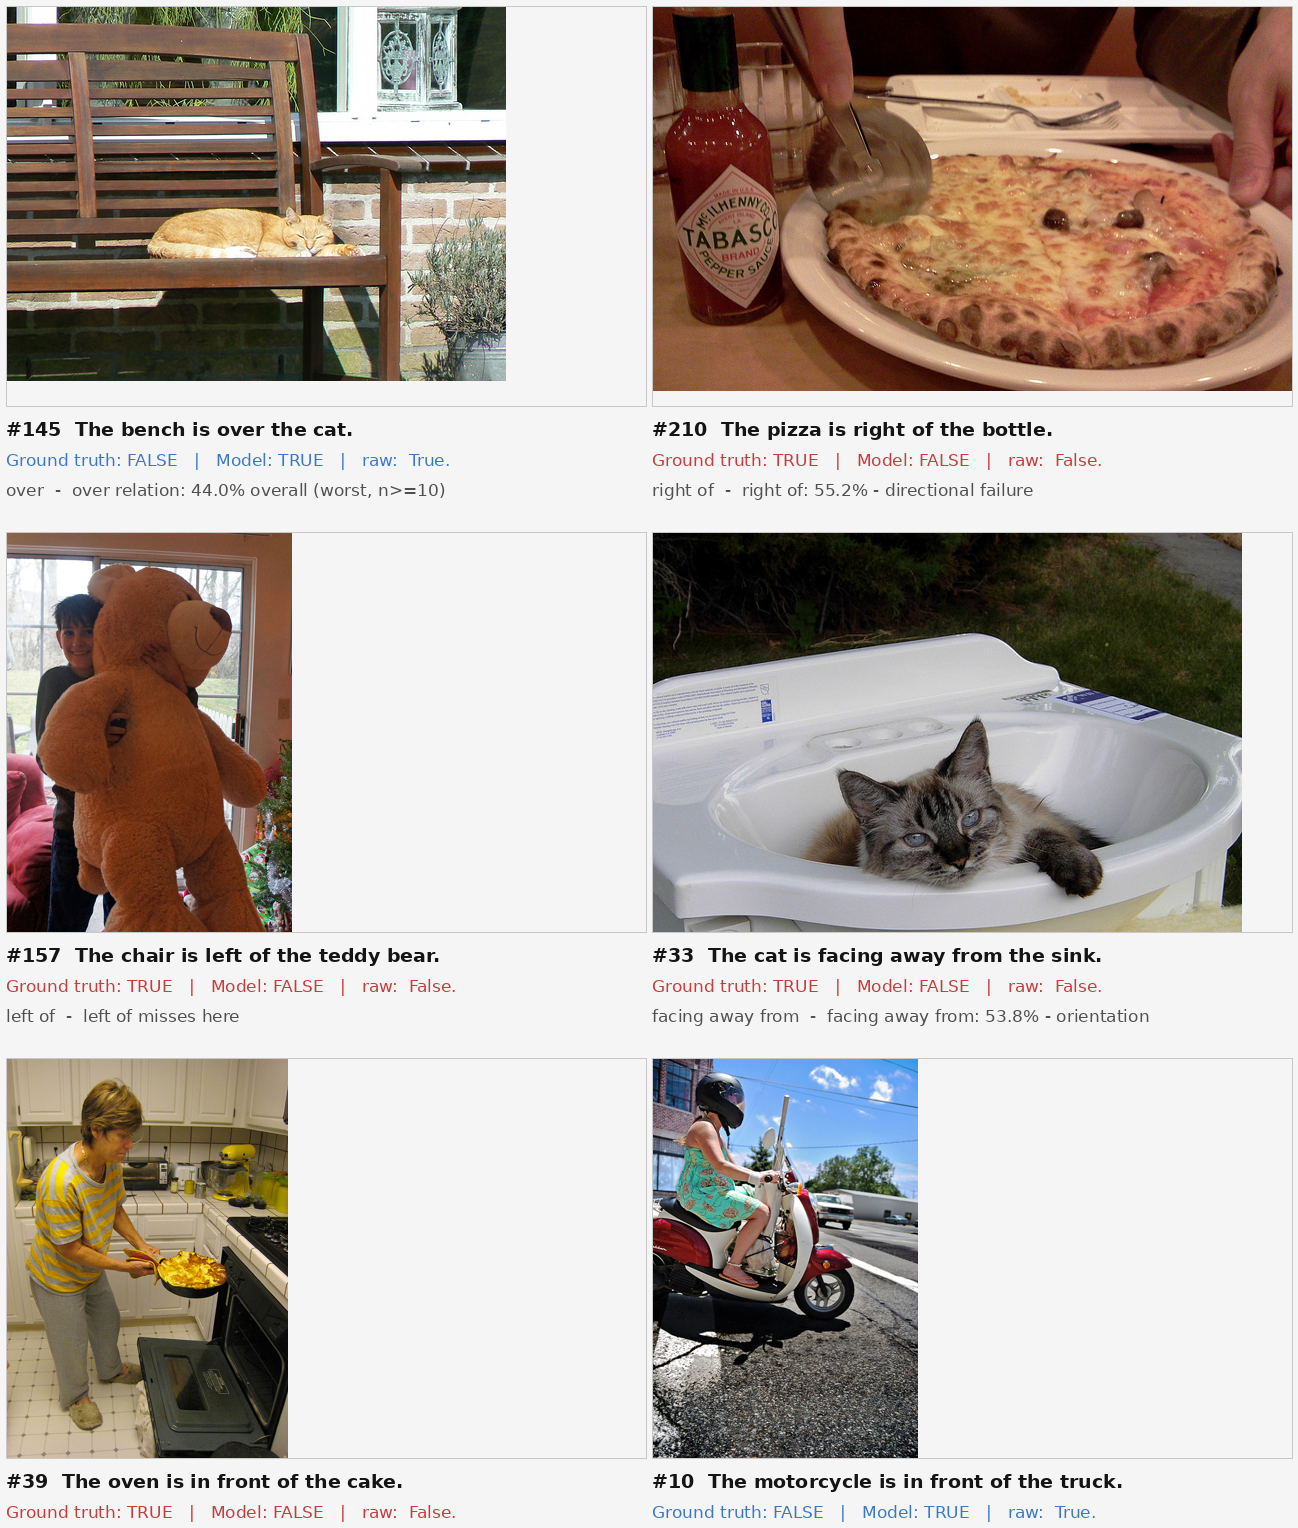
\includegraphics[width=\columnwidth]{fig/representative_failures.png}
\caption{Representative persistent failures (annotated grid; 15 cases).
Images: VSR test set. Per the single-annotator exploratory audit, the most
frequent class is \emph{clear-image reasoning failure}: the pose is visually
interpretable to a human and the model still errs.}
\label{fig:failures}
\end{figure}

\textbf{Transition counts.} Scaling (2B$\rightarrow$7B zero-shot): 28 both
wrong, 23 2B-wrong/7B-right, 22 2B-right/7B-wrong, 64 both right. Adaptation
(7B zero$\rightarrow$7B LoRA): 20 both wrong, 30 fixed, 27 broken, 60 both
right. Of the 48 annotated cases, hard-negative training fixes 5; 15 still
fail under all three 7B conditions. Facing/facing-away account for 68.8\% of
persistent failures.

% ============================================================
% G. Reproducibility and artifact index
% ============================================================
\section{Reproducibility and Artifact Index}
\label{app:repro}

Code: anonymized archive accompanying this submission (no external links). Every headline number in this
paper maps to a committed artifact; the audit script
\texttt{scripts/make\_paper\_figures.py} recomputes the main tables directly
from the raw prediction CSVs (output archived at
\texttt{paper/fig/audit\_output.txt}).

\begin{table*}[h]
\centering
\footnotesize
\setlength{\tabcolsep}{6pt}
\begin{tabular}{lll}
\toprule
Headline number & Artifact & Commit \\
\midrule
74.0 / 76.6 / 76.5 / 68.3 (2B) & \texttt{smolvlm2\_*\_metrics\_*.json} & --- \\
80.9 / 84.7 / 84.3 / 82.9 / 83.1 (7B) & \texttt{*\_metrics\_*.json} & --- \\
62.8 / 63.5 / 65.7 / 66.4 (orient.\ family) & same + prediction CSVs &
same \\
Per-relation cells (Table~1 (main)) & \texttt{orientation\_analysis.json} & --- \\
48-failure taxonomy & \texttt{orientation\_persistent\_*.json} & --- \\
Probe tables (App.~\ref{app:probes}) & \texttt{probe/*.json} & --- \\
Two-stage (App.~D, agreement-based rows 15--18) & \texttt{two\_stage\_results.json} & --- \\
Consistency (Fig.~4 (main)) & \texttt{consistency\_stats\_all.json} & --- \\
Vision-side p-values & \texttt{vision\_side\_comparison.json} & --- \\
SITE numbers & \texttt{site/zeroshot\_7b\_predictions.csv} & --- \\
 & \texttt{site/zeroshot\_image\_metrics.json} & \\
\bottomrule
\end{tabular}
\caption{Headline-number $\rightarrow$ artifact $\rightarrow$ commit index (all
paths relative to \texttt{results/}).}
\label{tab:artifacts}
\end{table*}

\textbf{Environments.} VSR/7B and SITE runs: Ubuntu 24.04, Python 3.12.13,
torch 2.12.1+cu130, transformers 5.14.1, datasets 5.0.1, peft 0.20.0, 1$\times$
RTX A6000 (48\,GB). 2B runs: earlier python3.10-era environment (SmolVLM2
wrapper). No lock files exist; the adapter configs (committed) pin the LoRA
hyperparameters. Seeds: 42 defaults in 2B paths; single default seed elsewhere
--- per-run seeds are not recorded in the metrics JSONs (a known limitation).

\textbf{Canonical freeze.} The experimental result set is frozen at tag
\texttt{paper-freeze-v1}. Canonical tables are generated by
\texttt{scripts/build\_canonical\_tables.py}; clean-label results by
\texttt{scripts/clean\_label\_orientation.py}; publication figures by
\texttt{scripts/make\_publication\_figures.py}; SITE paired transfer statistics
by \texttt{scripts/compare\_site\_zeroshot\_lora.py}; VSR/SITE headline
recomputation by \texttt{scripts/make\_paper\_figures.py} (output archived at
\texttt{paper/fig/audit\_output.txt}).

\textbf{Two-stage reproducibility caveat.} The two-stage pipeline requires
per-patch embeddings (\texttt{results/probe/patch\_embeddings.pkl}, 8.2\,GB,
not committed; regenerable on GPU via
\texttt{scripts/extract\_patch\_embeddings.py}) and hard-codes a Linux working
directory. The committed evidence is the aggregate
\texttt{results/two\_stage\_results.json} (agreement-based, see App.~D); the
per-example decisions are not committed.

\textbf{SITE secondary-subset audit note (corrected before submission).} An
earlier derived analysis (\texttt{compare\_site\_zeroshot\_lora.py} v1, which
fed the initial \texttt{zeroshot\_image\_metrics.json}-adjacent figures and the
first canonical site table) reconstructed the secondary subset by applying
\verb|ORIENTATION_KEYWORDS| to the \emph{question text only}, yielding
$n{=}1{,}824$ (47.3\% raw / 22.6\% CAA). The frozen protocol's preregistered
definition --- \texttt{results/site/site\_protocol.json}
$\rightarrow$ \texttt{frozen\_ids.secondary} (3{,}272 examples; 2{,}024 with
images), intersected with the 2{,}591 evaluated IDs --- is the authoritative
subset, and all numbers in this paper use it ($n{=}2{,}024$; zero-shot 48.3\% /
24.0\% CAA; VSR-LoRA 48.7\% / 24.5\%, $p{=}0.70$). The derived question-only
figure was corrected before submission; both definitions support the same
conclusion (orientation $\ll$ primary), but only the frozen-ID set matches the
preregistration. No prediction CSV was modified and no model was rerun.

\textbf{Data licenses/access.} VSR: \texttt{cambridgeltl/vsr\_random} (HF).
SITE: \texttt{franky-veteran/SITE-Bench}, CC-BY-4.0 (media in ~130\,GB zips;
requires HF read token). LoRA adapters are committed and loadable with peft;
base-model weights via HF Hub.

\textbf{Exact artifacts for the probe tables} (App.~\ref{app:probes}):
\texttt{results/probe/probe\_results.json},
\texttt{results/probe/patch\_probe\_results.json},
\texttt{results/probe/grounded\_probe\_results.json},
\texttt{results/probe/clear\_subset\_results.json},
\texttt{results/probe/grounded\_boxes.json}.
